\section{Modeling Mutation}\label{sec:mm}
In this section, we describe our proposed 3-parameter $\theta = \{ d, u, c\}$ mutation model.

\subsection{Repeat Unit Change Per Generation}\label{subsec:rucpg}
The simplest model of microsatellite mutation and evolution is the stepwise mutation
model of Ohta and Kimura~\cite{ohtaModelMutationAppropriate2007}.
Let $\lambda : \mathbb{Z}^+ \rightarrow \mathbb{Z}^+$ represent some function that accepts some repeat length and outputs some
repeat length.
Given a population $\pi_t$ at generation $t$ and some repeat length $\ell_t \in \pi_t$, the mutated repeat length
in the next generation $\lambda(\ell_{t}) = \ell_{t+1}$ takes three different states:
\begin{equation}
    \lambda(\ell_t) \in \{ \ell_t + 1 , \ell_t, \ell_t - 1\}
\end{equation}
Per generation, each microsatellite variant mutates up one repeat length (expansion), down one repeat length
(contraction), or stays the same -- all with equal probability.

Let $\mu_u$ represent the probability of upward mutation and $\mu_d$ represent the probability of downward mutation.
We can construct our function $\lambda$ as such:
\begin{enumerate}
    \item We are given some repeat length $\ell_t$, an upward mutation rate $\mu_u$, and a
        downward mutation rate $\mu_d$.
    \item Sample two numbers from a uniform random distribution: $x_u, x_d \sim U(0, 1)$.
    \item If $\mu_u > x_u$, then $\lambda(\ell_{t}) = \ell_t + 1$.
        This is the inverse transform sampling method. \label{enum:um}
    \item If $\mu_d > x_d$ but $\mu_u \leq x_u$, then $\lambda(\ell_{t}) = \ell_t - 1$. \label{enum:dm}
        If $\mu_d > x_d \ \land \ \mu_u > x_u$, then $\lambda(\ell_{t)} = \ell_{t}$.
\end{enumerate}

There does exist evidence that mutations occur at steps greater than one repeat length.
A model that takes this into account is the two-phase model, which follows the stepwise mutation model with probability
$p$ and mutates up and down with a length sampled from a geometric distribution, with probability $1-p$
~\cite{dirienzoMutationalProcessesSimplesequence1994}.
This is modeled by the procedure below:
\begin{enumerate}
    \item We are given some repeat length $\ell_t$, an upward mutation rate $\mu_u$, a
        downward mutation rate $\mu_d$, the probability of the stepwise mutation model $p$, and the success probability
        for the geometric distribution $m$.
    \item Sample three numbers from a uniform random distribution: $x_u, x_d, x_p \sim U(0, 1)$.
    \item If $p > x_p$, then we set the changes in repeat length $\Delta_u = 1, \Delta_d = 1$.
        Otherwise, we sample our changse in repeat length from a geometric distribution:
        $\Delta_u, \Delta_d \sim \mathit{Geom}(m)$.
    \item If $\mu_u > x_u$, then $\lambda(\ell_{t}) = \ell_t + \Delta_u$.
    \item If $\mu_d > x_d$ but $\mu_u \leq x_u$, then $\lambda(\ell_{t}) = \ell_t - \Delta_d$.
        If $\mu_d > x_d \ \land \ \mu_u > x_u$, then $\lambda(\ell_{t)} = \ell_{t} + \Delta_u - \Delta_d$.
\end{enumerate}

The two-phase model is more flexible here, but this introduces two new parameters to estimate: $p$ and $m$.
According to Sainudiin, the likelihood of all ``one phase'' models are
not significantly different than their two phase counterparts~\cite{sainudiinMicrosatelliteMutationModels2004}.
For this reason, our model restricts repeat lengths to mutate by at most one per generation.

\subsection{Mutation Rate Dependence on Repeat Unit}\label{subsec:mrdonru}
An assumption made with stepwise mutation model is that the probability of mutation is equal for all repeat lengths.

~\cite{kornbergEnzymaticSynthesisDeoxyribonucleic1964}.


TODO: (1) Mention the rate equality, (2) Mention the repeat length dependence on repeat unit,
(3) We are going with the repeat length dependence.

\subsection{Presence of Mutational Bias}\label{subsec:pomb}
TODO: (1) Mention the requirement of repeat length dependence, (2) Mention the constant bias parameter,
(3) Mention the linear bias, (4) Mention the focal bias

Our focal bias $\hat{\ell} $is defined as the point where $\mu_u$ and $\mu_d$ intersect:
\begin{equation}
    \hat{\ell} = \frac{-c}{\frac{d}{u} - d}
%    \begin{aligned}
%        \mu_u &= \mu_d \\
%        \frac{d}{u}\ell + c &= d\ell \\
%        (\frac{d}{u} - d)\ell &= -c \\
%        \ell &= \frac{-c}{\frac{d}{u} - d}
%    \end{aligned}
\end{equation}

\begin{figure}
    \centering{\pgfplotsset{compat=1.5}
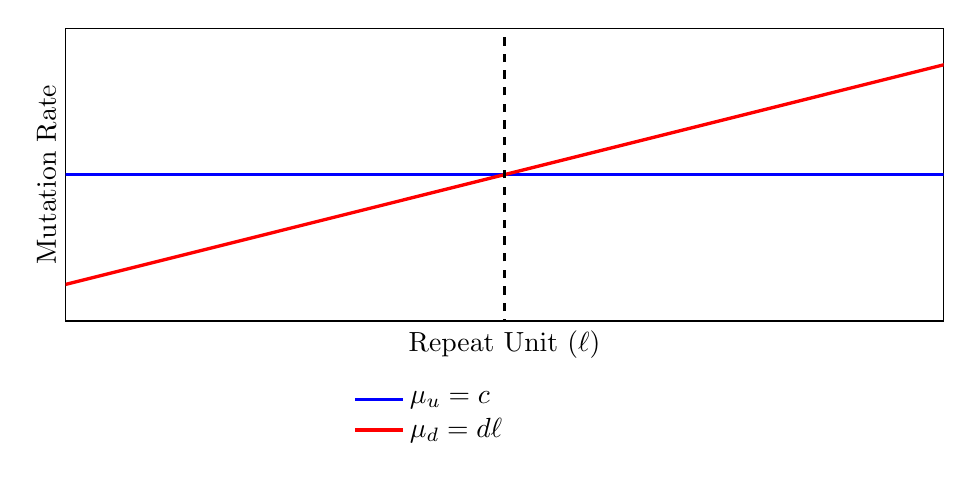
\begin{tikzpicture}
    \begin{axis}[
    width=1.05\linewidth, height=5.3cm,
    ylabel={Mutation Rate}, ymin=0.01, ymax=0.05,
    xlabel={Repeat Unit ($\ell$)}, xmin=6, xmax=18,
    xtick={0, 2, 4, 6, 8, 10, 12, 14, 16, 18, 20, 22, 24},
    samples=100, no markers, enlargelimits=false, legend style={at={(0.5,-0.2)},anchor=north,draw=none},
    legend cell align={left}, domain=0:25, ticks=none
    ]
        \addplot+[very thick]{0.03};
        \addlegendentry{$\mu_u = c$};

        \addplot+[very thick] {0.0025*x};
        \addlegendentry{\vspace*{5em}$\mu_d = d\ell$ \hspace*{5em}};

        \addplot+[very thick, black, dashed, forget plot] coordinates {(12, 0) (12, 0.05)};
    \end{axis}
\end{tikzpicture}}
    \caption{Our mutation model for $d=0.0025, u=1.2, c=0.005$.
    Our focal bias with these parameters is $\hat{\ell}=12$.}\label{fig:mutationModel}
\end{figure}